\subsection{Projeto Eletrônico}
\label{subsec:pro_eletronico}
% CIRCUITO ELÉTRICO/ELETRÔNICO COMPLETO
% MOSTRAR/EXPLICAR: PLACA DE CIRCUITO IMPRESSO DESENVOLVIDA
% TODO:
% ref:  https://produza.ind.br/gestao/pre-requisitos-tecnicos-para-montar-um-projeto-eletronico/

% \begin{figure}[H]
%     \centering
%     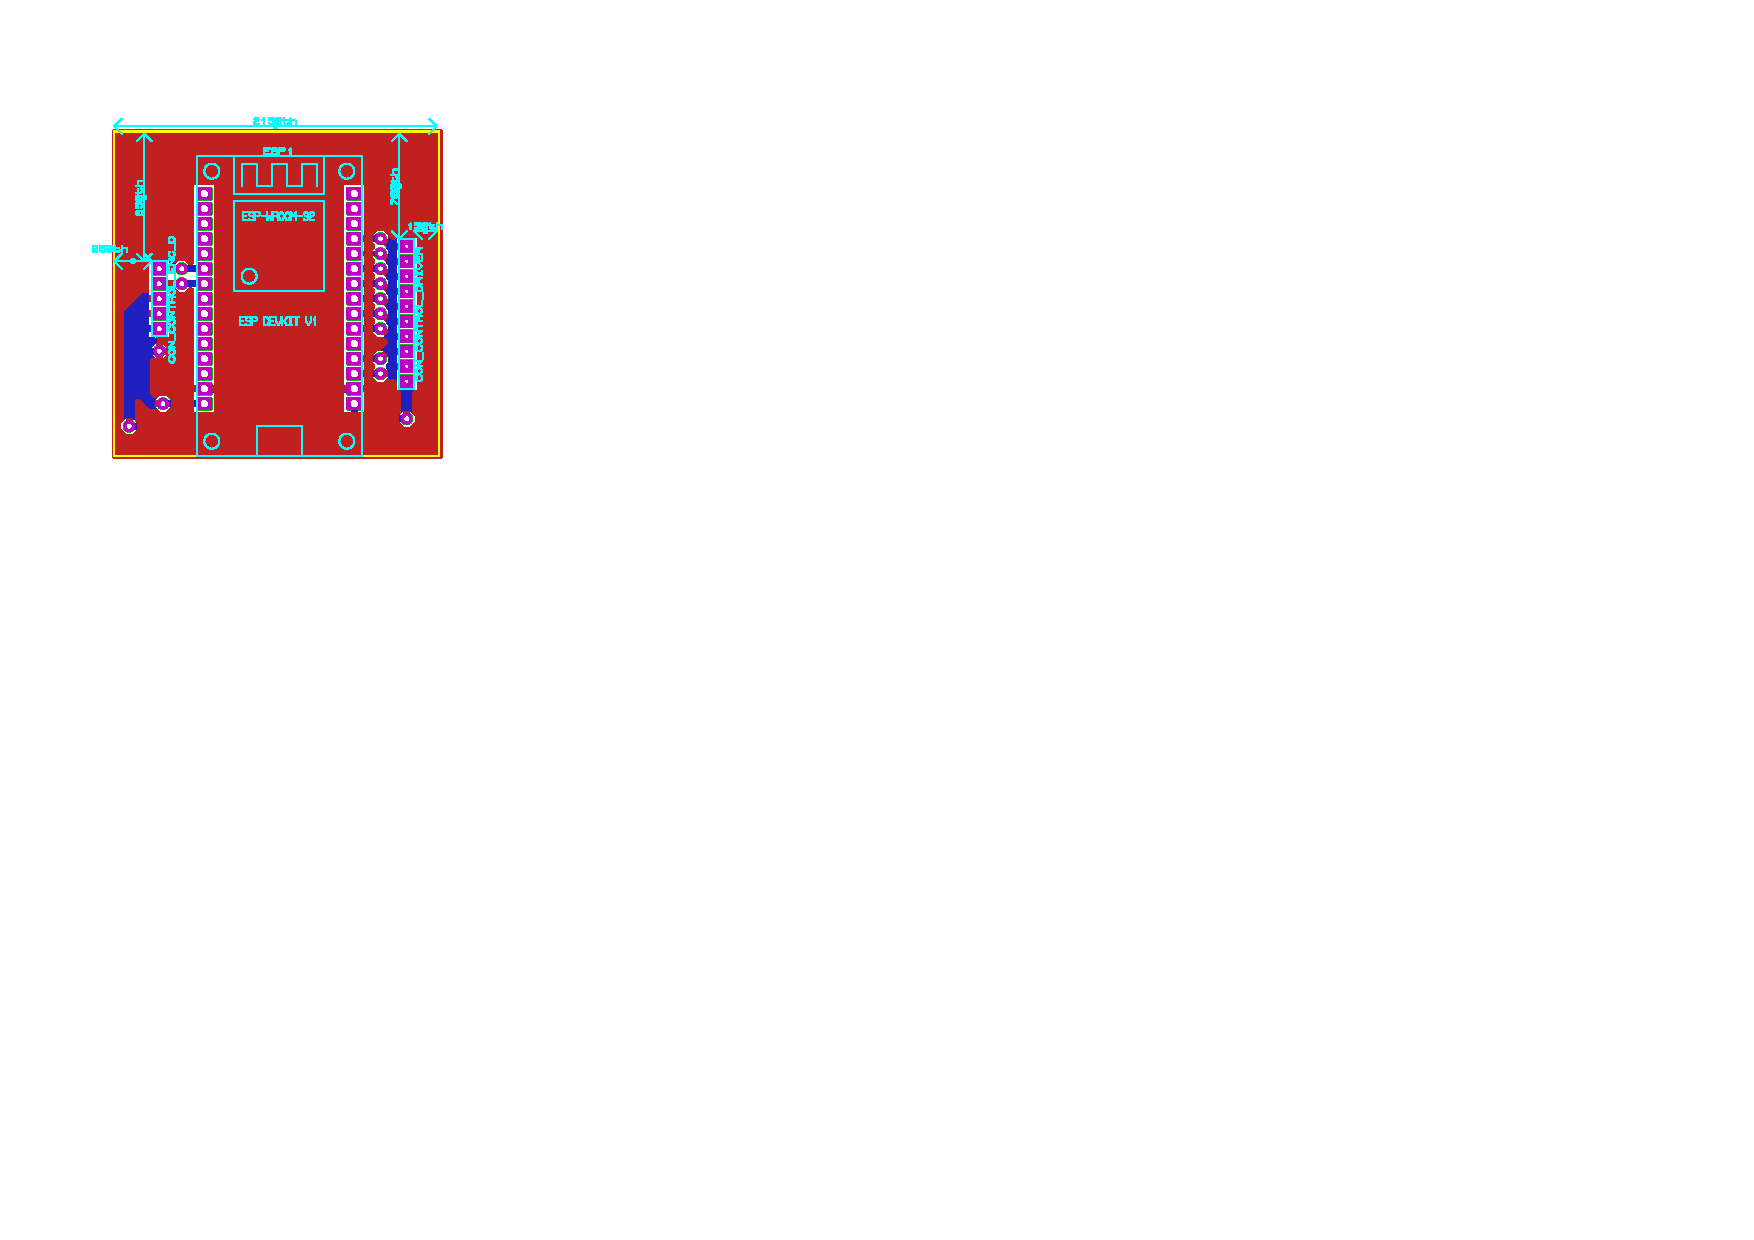
\includegraphics[width=\textwidth]{imagens/eletronica/placa/placa_controle_completa.pdf}
%     \caption{Caption}
%     % \label{fig:my_label}
% \end{figure}

% \begin{figure}[H]
%     \centering
%     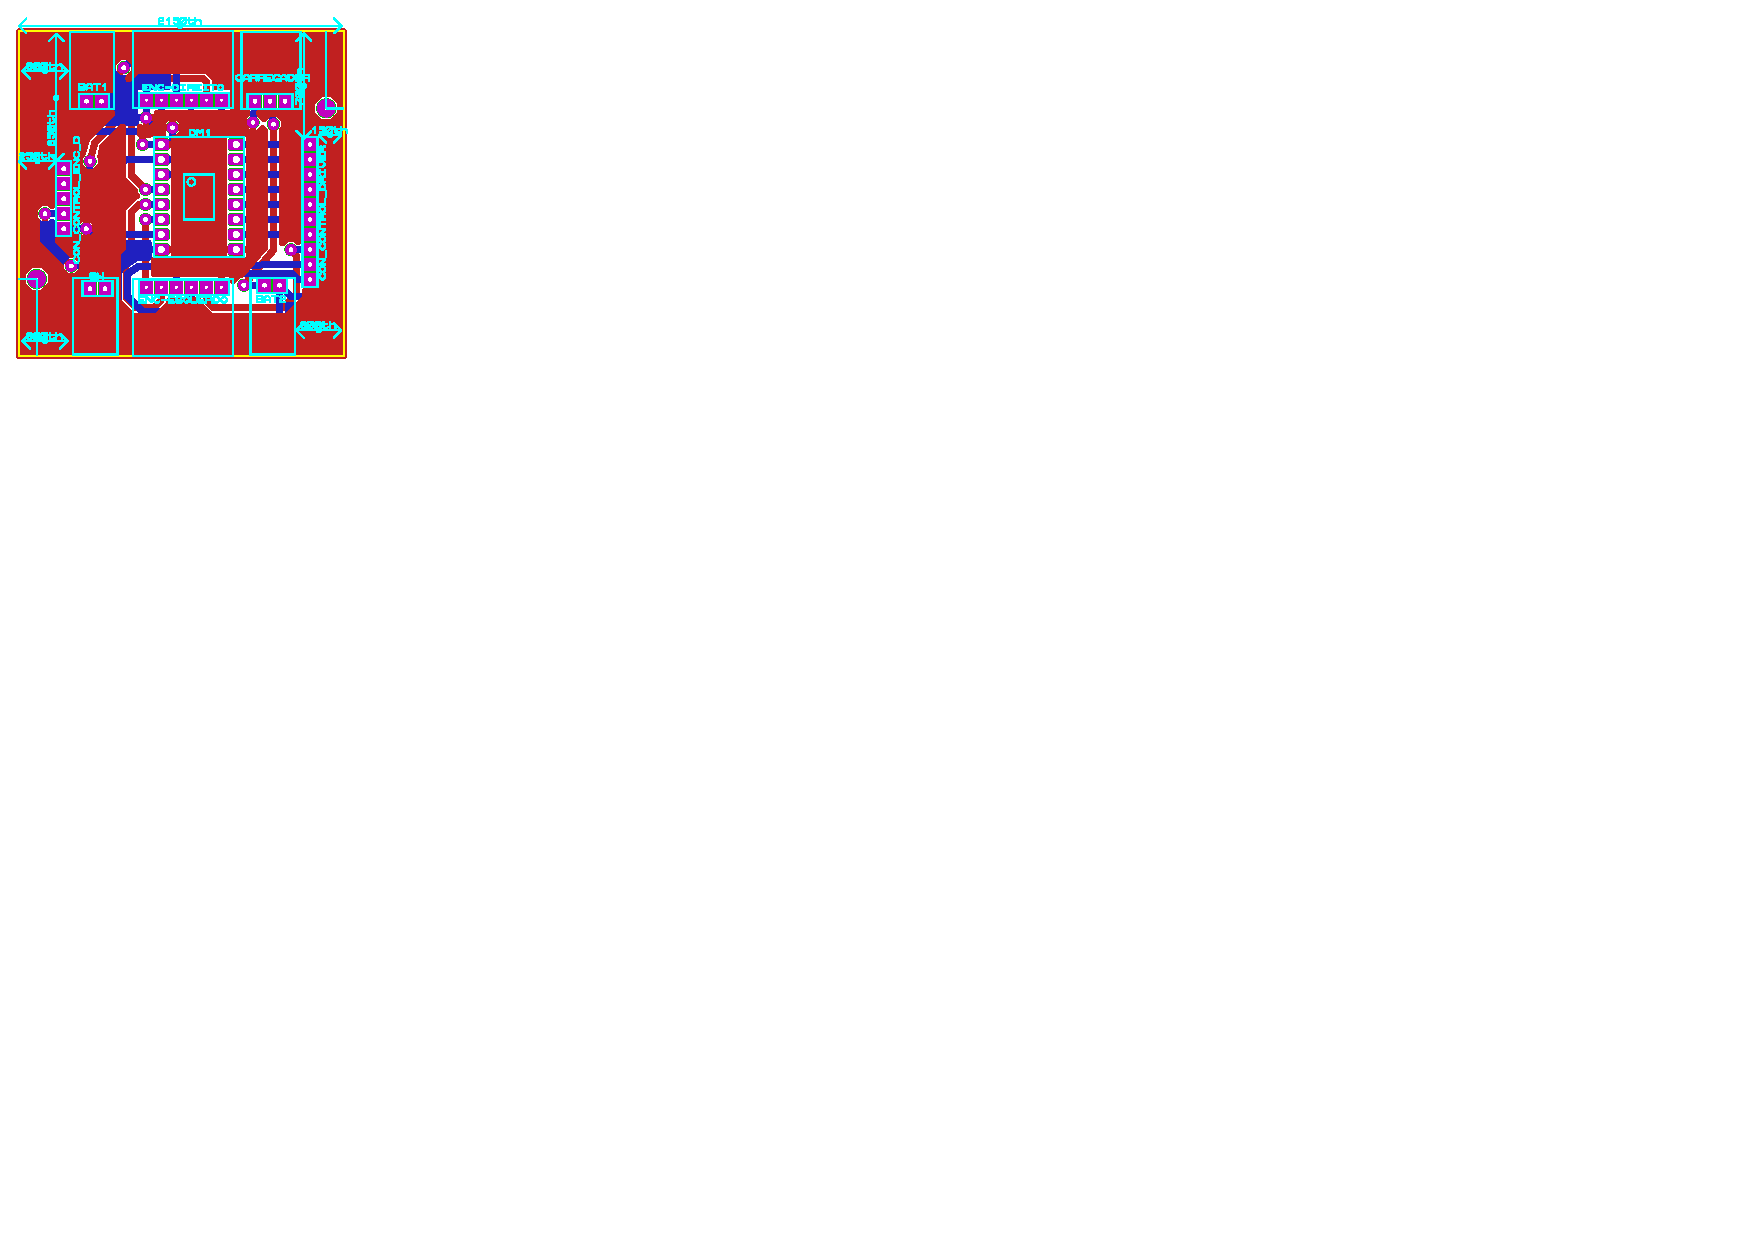
\includegraphics[width=\textwidth]{imagens/eletronica/placa/placa_driver_completa.pdf}
%     \caption{Caption}
%     % \label{fig:my_label}
% \end{figure}
O principal desafio por trás de se fazer uma placa de circuito eletrônico para esses robôs é acomodar os componentes, de forma a respeitar os limites das dimensões estabelecidos pela competição na qual os robôs serão utilizados (caber dentro de um cubo de $7,5$cm de aresta). A placa deve conter o microcontrolador, no seu kit de desenvolvimento, \textit{Driver motor} para acionamento dos motores CC, os \textit{Encoders} e ser alimentada por duas baterias de $1$ célula do tipo \textit{Lipo} (fornecendo assim uma alimentação de $7.4$V).\\


\begin{figure}[H]
    \centering
    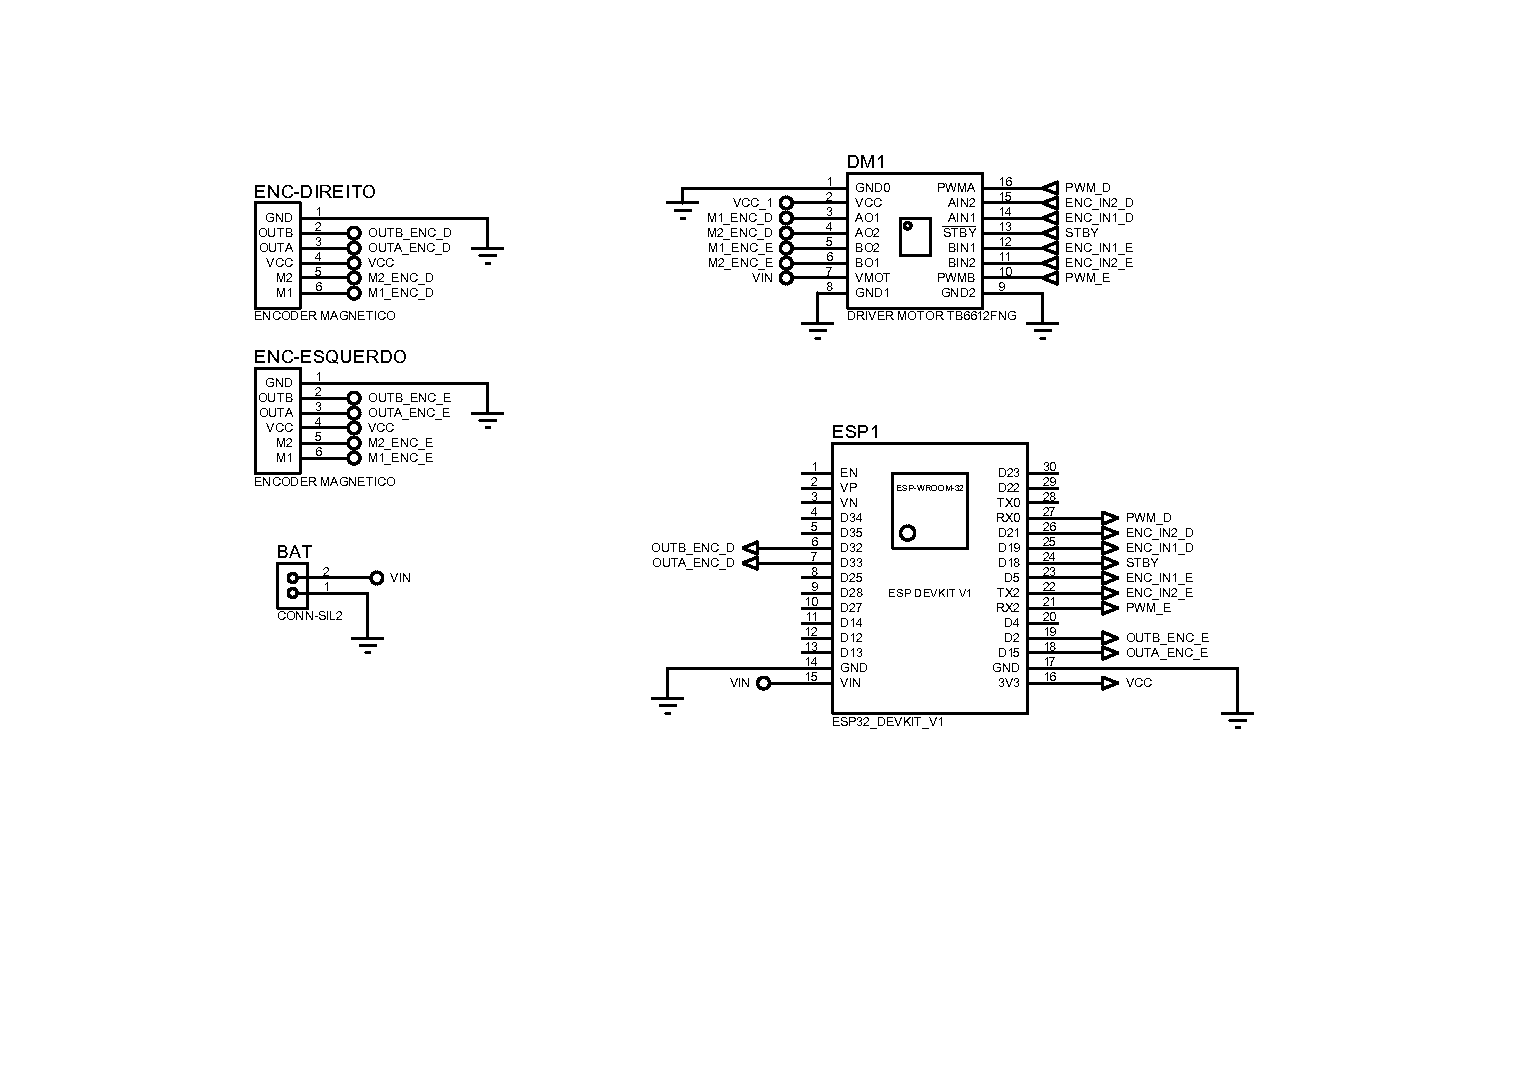
\includegraphics[width=\textwidth]{figuras/eletronica/placa/esquematico_completo.pdf}
    \caption{Diagrama esquemático do projeto eletrônico dos robôs.}
    \label{fig:diagrama_esquematico}
    \fonte{Própria.}
\end{figure}

A Figura \ref{fig:diagrama_esquematico} mostra o diagrama esquemático do sistema eletrônico utilizada nos robôs da equipe Poti. Uma descrição mais detalhada sobre os pinos e as nomenclatura utilizadas no diagrama é apresentado a seguir. 

\begin{itemize}
    \item \textbf{OUTA\_ENC\_(D ou E)}: Canal A do sinal de saída do \emph{Encoder} do motor direito (D) ou esquerdo (E).
    \item \textbf{OUTB\_ENC\_(D ou E)}: Canal B do sinal de saída do \emph{Encoder} do motor direito (D) ou esquerdo (E).
    \item \textbf{VCC}: Alimentação de $3.3$V proveniente da saída retificada pelo kit de desenvolvimento do ESP32.
    \item \textbf{VIN}: Alimentação de $7.4$V resultante da ligação em série das duas baterias Lipo de 1 célula.
    \item \textbf{M(1 ou 2)\_ENC\_(D ou E)}: Saída de alta potência ($7.4$V) vinda de um dos canais de saída \emph{Driver motor} (canal A ou B).
    \item \textbf{STBY}: Pino digital para habilitar ou desabilitar o \emph{Driver motor}.
    \item \textbf{ENC\_IN(1 ou 2)\_(D ou E)}: Pinos digitais que configuram o modo de operação da ponte H. Ou seja, controlam o sentido de rotação dos motores.
    \item \textbf{PWM\_(D ou E)}: Saída do $\mu{}C$ para o sinal PWM que regula a alimentação nos motores direito (D) e esquerdo (E).
\end{itemize}

% Este ponto foi o mais crítico nessa tarefa, devido à restrição de tamanho da placa ser de um quadrado com até $55$mm de lado. A solução adotada foi fazer em duas camadas, ou seja, duas placas cobreadas, ambas dupla face, dividindo os componentes. Em uma placa foi comportado o \textit{Driver}, bem como os conectores para os motores com os sensores e os conectores das baterias, e na outra apenas o microcontrolador. Para a conexão entre as placas foi utilizado um conector do tipo \textit{Head}, um macho e uma fêmea. Dessa forma, as placas conseguiram respeitar o limite dimensional e comportar todos os componentes necessários.